
\section{Experiments}
\label{SectionExperiment}
% Experiments
Our experiments were conducted on univariate data sets from the UCR archive as well as multivariate data sets from the UEA archive.
The data sets were chosen based on the criteria discussed in the subsection \ref{used data sets}.
Each of the data archives offers a train and test split of the data which we have used unchanged for all the classifiers.
All our experiments were run on a LINUX server with an AMD Ryzen 7 1700 Processor and 32GB RAM using Python 3.7.10.

We used the same experimental configuration through out all our experiments.
We fixed the value of the parameter $Splits$ = 10, that is for every data set the data would be revealed for the classifiers incrementally in batches of 10\% from the total length.
The chopping algorithm was set to always reveal data from the beginning of the time series.
Due to time limitations, we restricted our experiments to run only on the \nth{1}, \nth{2}, \nth{3} and \nth{10} chunksof the data sets by setting $ChunksToKeep$ = \{1,2,3,10\}.
We included the \nth{10} chunk to represent the baseline performance of each classifier if shown the full length data.
While the first 3 chunks were used to represent the classifiers in the early context scenarios.
Hyperparameters optimization was always carried out on all data sets with a $NumIterations$ maximum sampling value of 50 iterations, unless proven unfeasible for any of the classifiers due to memory shortage or time constraint.
In this case the experiment is repeated for all classifiers without hyperparameters optimization. We fixed the number of cross validation folds to 5.
The selected performance metric for our experiments was $Balanced Accuracy$.
Balanced accuracy is a performance metric which can handle data sets with skewed class distributions by avoiding inflated performance estimates.
To calculate balanced accuracy, the $Recall$ value is computed for each class then averaged over the total number of classes.
We have set all our experiments to use the same configuration for all classifiers on the same data set.


\subsection{Excluded Classifiers}
\label{SubsectionExcludedClassifiers}
Some of the included classifiers in the framework were excluded from our experiments; either because they couldn't operate in the early classification context
or because they couldn't attain comparable results to the published performances by previously published frameworks.

% Models excluded due not handling the context
For example, KNNED and InceptionTime were excluded due to the nature of their techniques which couldn't handle our created context.
Both algorithms are clearly able to learn on chopped training data sets.
However once the testing phase is reached, they would fail to classify instances of the testing data,
showing errors related to mismatches between the expeccted length of instances and the provided length.
Yet they would finish the last chunk where the data is provided in it's original full length.
The reason why KNNED fails such scenario, is that it uses ED which is a point-wise comparison distance measure that cannot compare time series of unequal lengths \cite{tan2019time}.
On the other hand, InceptionTime is a deep learning model whose input layer architecture, represented by number of nodes, depends on the length of the input time series \cite{fawaz2019deepreview}.
Since we use full length instances for testing, this caused an overflow of input data than what the model structure was expecting.
There have been literature discussing adapting TSCAs to unequal time series, but this is out of the scope of our experiments.
For more details refer to \cite{caiado2009comparison, tan2019time, fawaz2019deepreview}


% Models excluded due to implementation error
Although KNNDTW has been a competent time series classifier for decades; thanks to the exploitation of the elastic distance measure DTW.
We couldn't get either implementation of KNNDTW from $sktime$ and $pyts$ to work on the chopped data; due to errors in the data representation needed by lower level internal libraries.
KNNDTW would have been able to operate in the early classification context if used with a full warping window; which would have been successful in handling extreme classification cases like classifying full length data
even when learning on the 10\% chunk data set.


% Models excluded due to performance
Two classifiers were excluded because they attained significantly inferior results compared to the published scores; these are KNNMSM and LS.
Specially on the InsectWingbeatSound data set, for which we attained a difference in performance of -45.71\% for KNNMSM and -20.71\% for LS than the results published by \cite{bagnall2017great}

\subsection{Included Classifiers and Adjustments}
\label{SubsectionIncludedClassifiers}
% Models used
Our experiments proceeded with the remaining 5 classifiers; PForest, TSF, ST, CBOSS and WEASEL.
To focus only on the comparison of performance between classifiers and not preprocessing, we consider only data sets where all instances have the same length and no attributes have missing data.
We also focus our interest on data which is originally a timeseries data. This means that it is a collection of specific measurements across a span of time.
Which lead us to exclude some data set types from taking part in the experiment, more details are presented in subsection \ref{used data sets}.
We cover a total of 77 data sets from both the UR and the UEA archives, out of which 55 data sets are univariate and 22 data sets are multivariate.

Time and resources limitations played a big role shaping our experiments. Running classifiers is computationally expensive \cite{schafer2020teaser}
and takes up to hundreds of processing days.
This lead us to modify some algorithms to so that they can finish promptly; like in the case of PForest, or to use an enhanced version of the original
classifier with an option to control the learning phase time; like BOSS and ST.

Due to time limitations; We used the contractable implementations of BOSS and ST offered by $sktime$.
These implementations allows passing a time parameter which controls the sampling space for BOSS and the shapelets searching time for ST
beside other performance enhancements.
We set the value of the time contract for both to 60 minutes.
We have discussed the literature details of these enhancements for ST in subsection \ref{SubsubsectionST} and for BOSS in subsection \ref{SubsubsectionBOSS}.

We applied 2 adjustments to the PForest classifier.
Firstly, we excluded ED from the pool of distance measures that PForest selects from; since the ED has previously proven not to be compatible with our early classification context when used with the KNN classifier.
Secondly, we excluded TWE from the pool of distance measures when the size of the training data set exceeded 150 instances, which is the median of all data sets training sizes.
TWE is a very slow distance measure. It has been reported by \cite{bagnall2017great} to be the slowest among all elastic distance measures. When measured on classifing 10 test instances from the
StarlightCurves data set, it performed 10,000 times slower than ED.

\subsection{Learning weights for the $F_{\beta}-measure$}
\label{SubsectionLearningFBetaMeasure}
We use the $F_{\beta}-measure$ as an objective score for the performance of the classifiers.
The $F_{\beta}-measure$ has been a popular choice for evlauating eTSC algorithms \cite{schafer2020teaser} because of its
capacity to combine both earliness and accuracy.
Previous literature has always considered using a special case of the scoring function in which both earliness and accuracy contribute with the same weights.
This case is referred to as the Harmonic mean or the F-1 score and can be simply achieved by assigning the value of $\beta$ to 1.

For our experiments we conducted some experiments to decide if the use of equal weights for accuracy and earliness best suits our newly created context.
We experimented with the harmonic mean (i.e. $\beta$ = 1) like the previous papers and plotted the distribution of values for $F_{\beta}-measure$.
Figures \ref{fig:FBeta1} show a comparison between the distribution of values of $F_{1}$ and the distribution values of $Balanced Accuracy$ for CBoss.
The boxplots from the accuracy image shows that CBoss on the full length of the data has a median value of \textbf{0.829}, while on the 10\% data it shows a median value of \textbf{0.44}.
The two boxes do not overlap which means that there is a significant difference in the scores of the two versions.
What we would like for the $F_{\beta}-measure$ in this scenario, is to give a privilege for the 10\% version of the classifier as it learns on less training data, such that it would have
a high score if it can score a balanced accuracy close to that of the 100\% version.


\begin{figure}[!htbp]
  \captionsetup{justification=raggedright}
  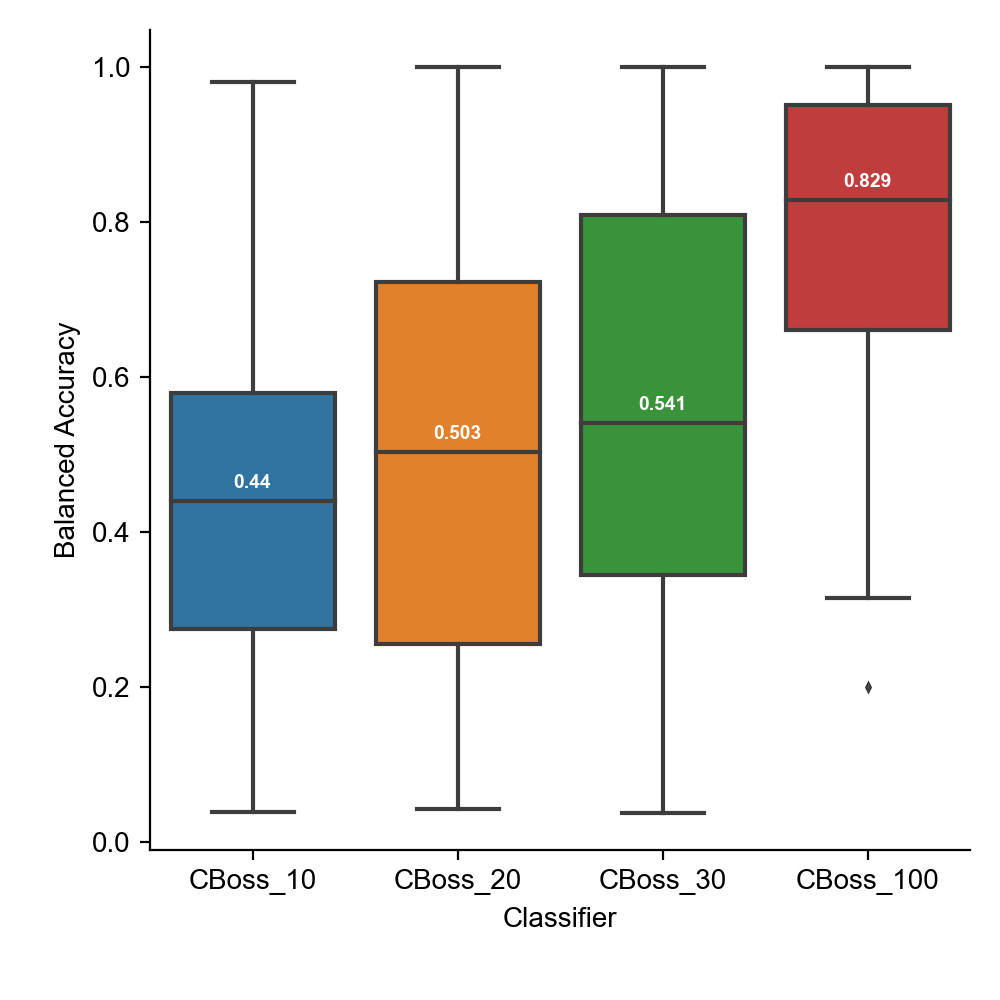
\includegraphics[width=0.49\textwidth,keepaspectratio]{boxplot_accuracy_CBoss.png}
  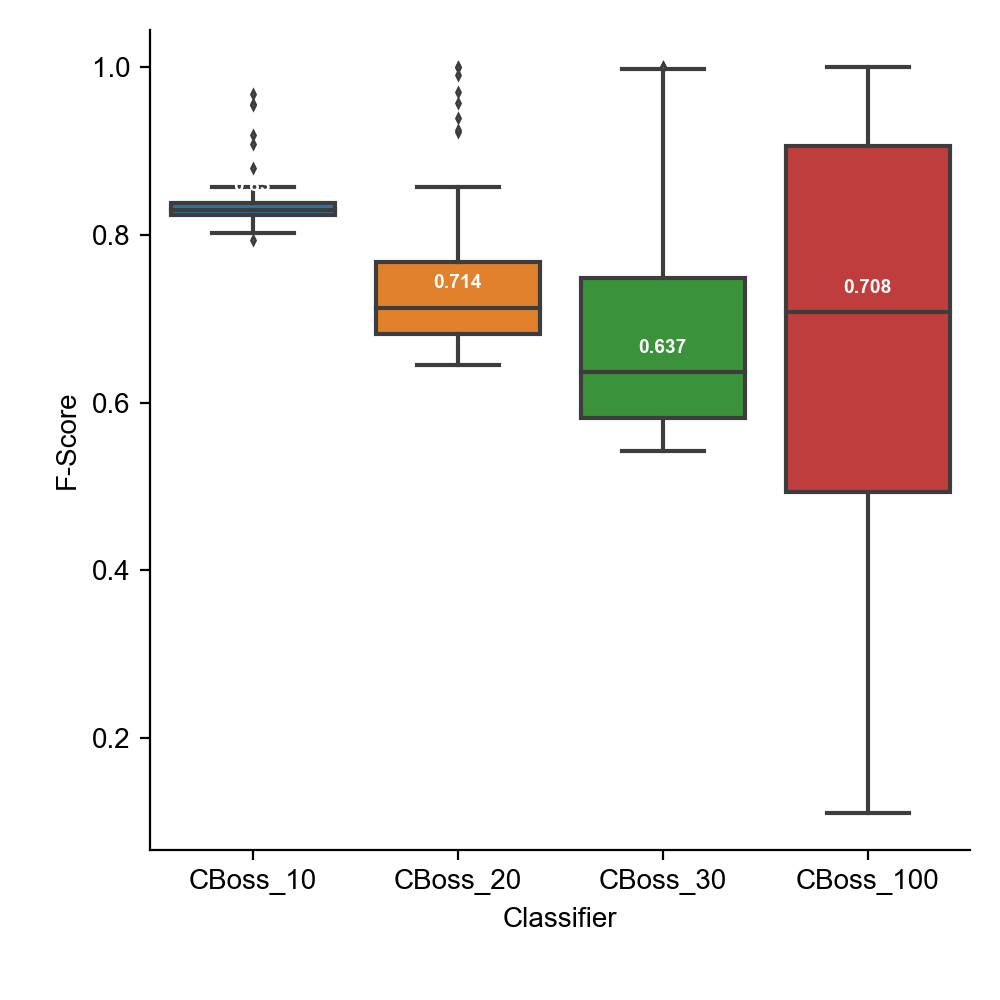
\includegraphics[width=0.49\textwidth,keepaspectratio]{boxplot_f_score_1_CBoss.png}
  \caption{Comparison between Balanced Accuracy (left) and $F_{1}$ (right) for CBoss}
  \label{fig:FBeta1}
\end{figure}

By checking the boxplots for the $F_{1}$, we find that the median value for the 10\% version is \textbf{0.83}, while the median value of the 100\% version is \textbf{0.708}.
Also the distribution of the values for the 10\% version is very close to the median and the minimum value is higher than the median of the 100\% version.
Which means that even for the data sets on which the 10\% version of CBoss scores very low accuracy scores, it will still get a high $F_{1}$ relative to the 100\% version.
The harmonic mean over-compensates for the lower accuracy scores with very high values for earliness causing misleading values.

To decide which $\beta$ value is best to use, we carried out a sequence of experiments using $\beta$ = [0.1, 0.9].
The value that gave the most reasonable results was 0.5.
Figure shows the same comparison between the boxplots of $Balanced Accuracy$ and $F_{\beta}-measure$ for CBoss but with $\beta$ = 0.5.
Still $F_{1}$ allows for compensation between accuracy and earliness for the 10\% version, but it refines the values.
The median value for the 10\% version became \textbf{0.705} while that of the 100\% is \textbf{0.795}.
The distribution of values for the 10\% is spread more and the maximum value is falling near the median value of the 100\%.

\begin{figure}[!htbp]
  \captionsetup{justification=raggedright}
  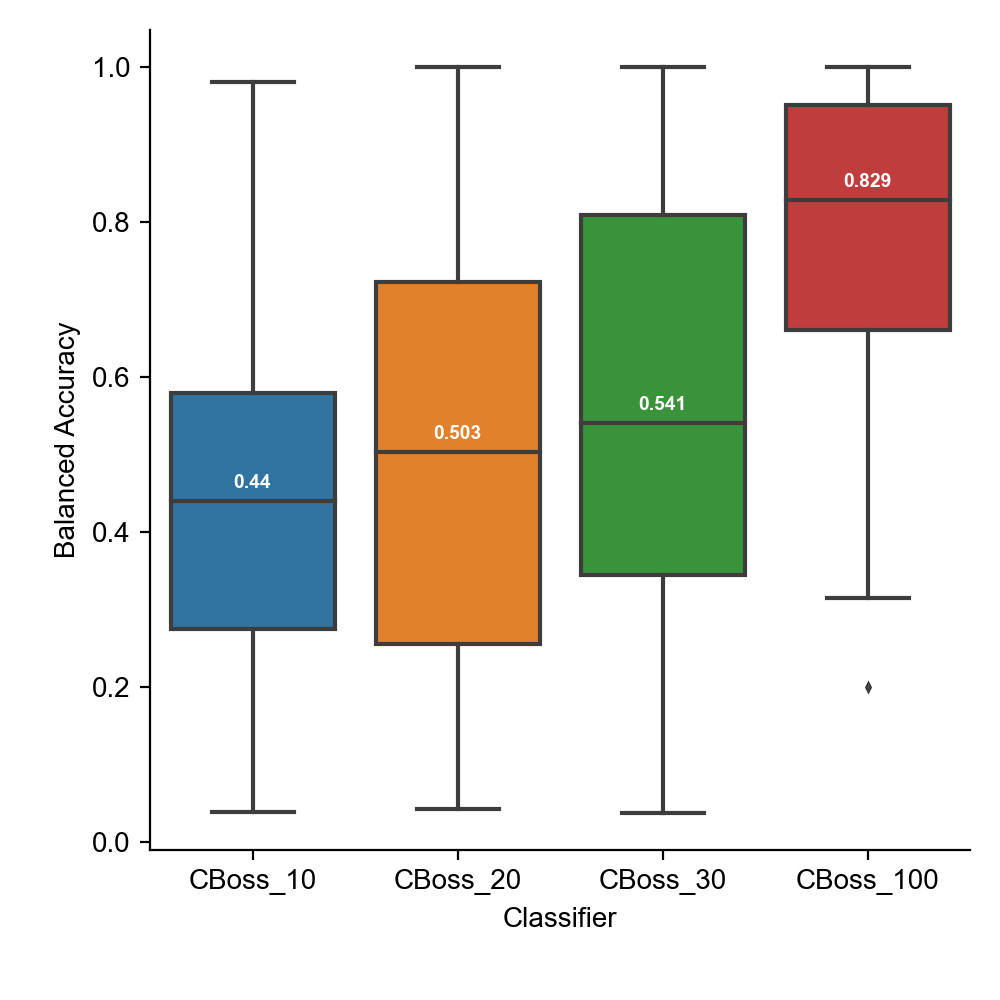
\includegraphics[width=0.49\textwidth,keepaspectratio]{boxplot_accuracy_CBoss.png}
  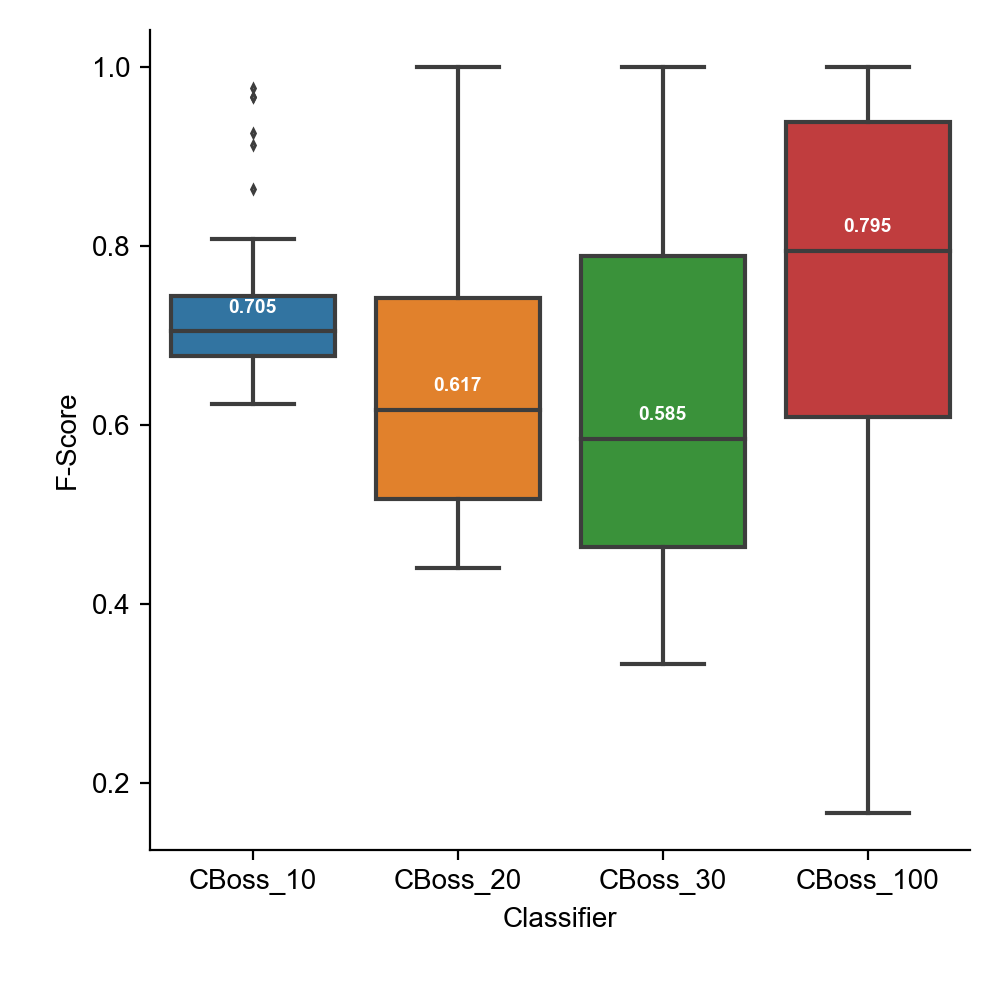
\includegraphics[width=0.49\textwidth,keepaspectratio]{boxplot_f_score_05_CBoss.png}
  \caption{Comparison between Balanced Accuracy (left) and $F_{0.5}$ (right) for CBoss}
  \label{fig:FBeta1}
\end{figure}

We believe that selecting the best value of $\beta$ is not trivial.
It is problem dependant and not one specific value can fit for all problems.
For our experiments we decided to give earliness less priority than performance,
but in other situations it might be the case that both of them contribute with the same importance or even earliness is more critical.



